\documentclass[conference]{IEEEtran}
\usepackage{cite}
\usepackage{amsmath,amssymb,amsfonts}
\usepackage{algorithmic}
\usepackage{graphicx}
\usepackage{textcomp}
\usepackage{xcolor}
\usepackage{hyperref}
\usepackage{tikz}
\usetikzlibrary{shapes.geometric, arrows, positioning}

% Configuração para exibir TABELA em português no padrão IEEE
\renewcommand{\tablename}{TABELA}

\def\BibTeX{{\rm B\kern-.05em{\sc i\kern-.025em b}\kern-.08em
    T\kern-.1667em\lower.7ex\hbox{E}\kern-.125emX}}

\IEEEoverridecommandlockouts

\begin{document}

\title{Análise Topológica de Redes de Colaboração no Rock Alternativo (1980--1990): Investigação de Propriedades de Mundo Pequeno, Escala Livre e Backbones de Produção\thanks{O código-fonte completo, a base de dados e a aplicação web interativa estão disponíveis no repositório GitHub: \url{https://github.com/PedroHSC-0/Analise-de-redes-rock-alternativo}}}

\author{\IEEEauthorblockN{1\textsuperscript{st} Pedro H. S. C.}
\IEEEauthorblockA{\textit{Departamento de Computação e Engenharia} \\
\textit{CEFET-MG -- Campus V}\\
Divinópolis, MG, Brasil \\
GitHub: \url{https://github.com/PedroHSC-0/Analise-de-redes-rock-alternativo}}
\and
\IEEEauthorblockN{2\textsuperscript{nd} Prof. Michel Pires da Silva}
\IEEEauthorblockA{\textit{Orientador - Dept. de Computação} \\
\textit{CEFET-MG / UFCI-MG}\\
Belo Horizonte, Brasil}
}

\maketitle

\begin{abstract}
Redes de colaboração artística constituem sistemas complexos cujas propriedades topológicas moldam a transmissão de influências culturais e a evolução de movimentos estéticos. Este trabalho apresenta uma investigação científica sobre a estrutura da rede de colaborações do Rock Alternativo das décadas de 1980 e 1990, empregando conceitos da Teoria dos Grafos e da Ciência das Redes Complexas. O domínio foi modelado computacionalmente como um grafo ponderado não-direcionado heterogêneo $G=(V, E, W)$, englobando $N=889$ vértices e $M=954$ arestas. Para integrar a frequência de parcerias com o impacto crítico das obras, formulou-se uma função de ponderação híbrida $W_{\text{híbrido}} = \alpha \cdot \bar{W}_{\text{bruto}} + (1-\alpha) \cdot \bar{Q}_{\text{crítica}}$, acompanhada pela extração do \textit{backbone} multiescala via Filtro de Disparidade (\textit{Disparity Filter}, Serrano et al., 2009). Os resultados empíricos comprovaram que a rede exibe comportamento de \textbf{Mundo Pequeno} (Índice Watts-Strogatz $S = 6,60 > 1,0$), curto caminho médio ($L = 9,3669$) e distribuição de graus em \textbf{Lei de Potência} ($\gamma = 1,409, R^2 = 0,7944$), caracterizando uma rede de \textbf{Escala Livre}. A análise de centralidade de intermediação (\textit{Betweenness Centrality}) revelou que produtores musicais e engenheiros de som (como Brian Eno, $C_B = 0,3188$, Dave Fridmann, $C_B = 0,2197$, e John Cale, $C_B = 0,1713$) atuam como pontes estruturais indispensáveis, unindo comunidades estéticas isoladas (Modularidade de Louvain $Q = 0,9003$) e garantindo a coesão global do ecossistema alternativo.
\end{abstract}

\begin{IEEEkeywords}
Teoria dos Grafos, Redes Complexas, Mundo Pequeno, Escala Livre, Filtro de Disparidade, Rock Alternativo, CEFET-MG Divinópolis.
\end{IEEEkeywords}

\section{Introdução}

A Ciência das Redes Complexas consolidou-se nas últimas décadas como um paradigma interdisciplinar fundamental para a compreensão da estrutura, dinamismo e resiliência de sistemas reais \cite{barabasi1999}. Ao abstrair entidades como vértices e suas interações como arestas em uma representação matemática $G=(V, E)$, essa abordagem revelou que sistemas de naturezas profundamente distintas --- desde infraestruturas físicas de transporte e redes neurais biológicas até plataformas de interação digital e circuitos de coautoria profissional --- compartilham propriedades estatísticas e organizacionais universais \cite{watts1998}.

No âmbito da sociologia da cultura e da economia criativa, a formação de alianças artísticas entre músicos, bandas e produtores de áudio desempenha um papel determinante na gestação, maturação e difusão de novos movimentos estéticos \cite{gleiser2003}. Longe de ser fruto do acaso ou da ação isolada de indivíduos genializados, a inovação artística emerge de complexas teias sociotécnicas. Nessas redes, convenções sonoras, timbres em estúdio, arranjos e identidades visuais são continuamente negociados, mesclados e transmitidos através das fronteiras geográficas e estilísticas.

Durante as décadas de 1970, 1980 e 1990, a indústria fonográfica mundial passou por uma transição sociotécnica profunda. Até meados dos anos 1970, a produção musical era estritamente corporativa, centralizada e hierarquizada pelas grandes gravadoras (\textit{major labels} --- tais como CBS/Columbia, Warner, RCA, EMI e PolyGram). O modelo tradicional funcionava por controle \textit{top-down}: executivos e selos monopolizavam o agendamento de estúdios, os orçamentos de gravação, os canais de distribuição física e as programações de rádio, impondo um padrão de produção altamente organizado no plano empresarial, porém esteticamente conservador e rígido.

Em contraposição a esse hegemonismo corporativo, o surgimento do Punk e a subsequente explosão do Rock Alternativo nos anos 80 e 90 (abrangendo vertentes como o \textit{Grunge}, o \textit{Post-Punk}, o \textit{Shoegaze}, o \textit{Britpop}, o \textit{Industrial} e o \textit{Indie Rock}) instauraram a ética autônoma do \textit{Do-It-Yourself} (DIY / ``Faça Você Mesmo''). Essa nova postura descentralizou a produção musical por meio de selos independentes (\textit{Sub Pop, Factory Records, Creation Records, SST Records, Dischord Records}), gravadores artesanais de fita cassete, estúdios comunitários e circuitos de turnês compartilhadas.

Todavia, essa transição para a autonomia estética suscita uma questão teórica e sociológica fundamental: ao romper com o controle centralizado das \textit{major labels}, a rede de colaborações do Rock Alternativo evoluiu como um sistema verdadeiramente caótico, desorganizado e estocástico, ou seguiu uma arquitetura topológica velada e altamente coesa? À primeira vista, o discurso libertário e a pulverização do movimento DIY sugeririam uma estrutura anárquica e fragmentada em aglomerados isolados. Por outro lado, a hipótese central deste trabalho é de que o ecossistema alternativo substituiu a hierarquia corporativa por uma rede complexa autorregulada, na qual determinados vértices articuladores --- em especial os produtores musicais e engenheiros de som --- atuaram como pontes críticas de intermediação informacional e estética.

Neste trabalho, desenvolvido no contexto da disciplina de \textit{Estruturas em Árvores e Teoria dos Grafos} do CEFET-MG (Campus V, Divinópolis), sob orientação do Prof. Michel Pires da Silva, propõe-se uma investigação computacional minuciosa sobre a rede de colaborações do Rock Alternativo dos anos 80 e 90. Modelou-se um grafo ponderado heterogêneo $G=(V, E, W)$ composto por $N=889$ vértices e $M=954$ arestas, no qual bandas, músicos solo e produtores são diferenciados por atributos taxonômicos e cujas arestas incorporam tanto o volume bruto de colaborações quanto o reconhecimento crítico das obras produzidas.

O objetivo principal deste artigo é demonstrar empiricamente que a rede possui comportamento de Mundo Pequeno (\textit{Small-World}) e Escala Livre (\textit{Scale-Free}), investigando como o Filtro de Disparidade (\textit{Disparity Filter}) e a análise de intermediação (\textit{Edge \& Node Betweenness Centrality}) evidenciam o papel estruturante dos produtores na preservação da coesão do grafo.

Para alcançar este objetivo, o artigo está estruturado em cinco seções principais: a Seção II apresenta o Referencial Teórico e a fundamentação matemática adotada; a Seção III detalha a Metodologia e a modelagem computacional da solução; a Seção IV discute criticamente os Resultados e métricas topológicas obtidas; e a Seção V expõe as Conclusões e perspectivas para trabalhos futuros.

\section{Referencial Teórico e Estado da Arte}

O estudo formal de redes de colaboração repousa sobre a Teoria dos Grafos Ponderados. Um grafo ponderado não-direcionado é formalmente definido pela tupla $G = (V, E, W)$, em que $V$ representa o conjunto de vértices de cardinalidade $|V| = N$, $E \subseteq V \times V$ representa o conjunto de arestas de cardinalidade $|E| = M$, e $W: E \to \mathbb{R}^+$ é a função de ponderação que atribui uma intensidade escalar $w_{ij} > 0$ a cada conexão entre os nós $i, j \in V$. 

Na caracterização da importância estrutural de vértices e arestas, destacam-se o grau de um nó $k_i = \sum_{j \in N(i)} 1$, sua força escalar $s_i = \sum_{j \in N(i)} w_{ij}$, e a centralidade de intermediação de arestas (\textit{Edge Betweenness Centrality}), formulada por Girvan e Newman \cite{girvan2002} para quantificar a fração de caminhos mínimos de informação que atravessam uma determinada aresta $e \in E$:

\begin{equation}
C_B(e) = \sum_{s \neq t \in V} \frac{\sigma_{st}(e)}{\sigma_{st}}
\end{equation}

em que $\sigma_{st}$ representa o número total de caminhos mínimos entre os vértices $s$ e $t$, e $\sigma_{st}(e)$ denota a quantidade daqueles caminhos que contêm a aresta $e$. Arestas que apresentam elevados valores de $C_B(e)$ atuam como pontes topológicas críticas, cuja desconexão ocasiona o aumento expressivo do diâmetro do grafo ou sua fragmentação em componentes isolados.

A topologia de redes reais afasta-se notavelmente dos modelos de grafos aleatórios clássicos propostos por Erdős e Rényi (1959). Watts e Strogatz \cite{watts1998} introduziram a classe das redes de \textbf{Mundo Pequeno} (\textit{Small-World Networks}), caracterizadas por apresentar um elevado coeficiente de aglomeração local ($C$), que reflete a densa formação de triângulos em agrupamentos sociais, concomitantemente a uma distância média de caminho mínimo ($L$) reduzida entre pares arbitrários de nós. A quantificação rigorosa dessa propriedade é realizada pelo Índice Watts-Strogatz ($S$), que compara o desempenho do grafo observado com o de uma rede aleatória equivalente equipada com o mesmo número de nós e arestas:

\begin{equation}
S = \frac{C / C_{\text{rand}}}{L / L_{\text{rand}}}
\end{equation}

Redes que exibem $S > 1,0$ são formalmente classificadas como estruturas de Mundo Pequeno, indicando que a propagação de influências e informações ocorre de maneira altamente eficiente por meio de conexões de alcance global.

Simultaneamente, Barabási e Albert \cite{barabasi1999} identificaram as redes de \textbf{Escala Livre} (\textit{Scale-Free Networks}), cujas distribuições de graus $P(k)$ obedecem a uma taxa de decaimento assintótico segundo uma Lei de Potência:

\begin{equation}
P(k) \sim k^{-\gamma}
\end{equation}

em que $\gamma$ é o expoente característico da escala. Essa distribuição assimétrica emerge tipicamente pelo princípio da conexão preferencial (\textit{preferential attachment}), no qual novos vértices tendem a se conectar predominantemente a nós que já possuem elevadas contagens de conexões (\textit{hubs}). Na indústria da música, esse mecanismo traduz-se no fenômeno sociológico em que bandas emergentes buscam ativamente gravar com produtores renomados ou integrar selos de grande visibilidade.

No estado da arte da análise computacional de redes musicais, destacam-se os trabalhos pioneiros de Gleiser e Danon \cite{gleiser2003}, que examinaram a estrutura de comunidades no Jazz, e de Park, McDermott e Mace \cite{park2007}, que aplicaram Teoria dos Grafos para mapear a evolução estilística da música ocidental. Newman \cite{newman2001} já havia demonstrado que redes de coautoria científica e artística organizam-se em aglomerados modulares coesos unidos por indivíduos articuladores.

Entretanto, uma limitação frequente em pesquisas sobre redes ponderadas reside na estratégia de poda de arestas (\textit{graph pruning}). Métodos ingênuos baseados em corte de peso fixo ($w_{ij} < w_{\text{corte}}$) costumam eliminar conexões de menor peso mas essenciais para a conectividade local, isolando nós de menor grau. Para contornar essa vulnerabilidade, Serrano, Boguñá e Vespignani \cite{serrano2009} desenvolveram o \textbf{Filtro de Disparidade} (\textit{Disparity Filter}). Esse algoritmo estocástico preserva a espinha dorsal multiescala do grafo ao testar a hipótese nula de que os pesos das arestas incidentes em um nó $i$ de grau $k_i$ estão distribuídos uniformemente. A probabilidade observada $\alpha_{ij}$ de uma aresta possuir a fração de peso $x_{ij} = w_{ij} / s_i$ sob a hipótese nula é dada por:

\begin{equation}
\alpha_{ij} = (1 - x_{ij})^{k_i - 1}
\end{equation}

Arestas que satisfazem a condição $\alpha_{ij} < p_{\text{corte}}$ são mantidas no \textit{backbone} estatístico, preservando a integridade das pontes de intermediação independentemente da escala absoluta de suas forças.

Adicionalmente, a identificação de agrupamentos funcionais é realizada pelo Algoritmo de Louvain para \textbf{Detecção de Comunidades} \cite{blondel2008}. O método baseia-se na otimização da função de Modularidade ($Q$), definida como:

\begin{equation}
Q = \frac{1}{2m} \sum_{i,j} \left[ w_{ij} - \frac{k_i k_j}{2m} \right] \delta(c_i, c_j)
\end{equation}

em que $m = \frac{1}{2}\sum_{i,j} w_{ij}$ representa a soma total dos pesos das arestas do grafo, $c_i$ indica a comunidade atribuída ao vértice $i$, e $\delta(c_i, c_j)$ denota a função delta de Kronecker (que assume valor $1$ se $c_i = c_j$ e $0$ caso contrário). A maximização de $Q$ permite revelar como os subgêneros do Rock Alternativo se segregam em comunidades estéticas e de que maneira essas comunidades interagem.

\section{Metodologia e Modelagem Computacional}

A condução deste trabalho baseou-se em um pipeline rigoroso de engenharia de dados, modelagem computacional em Teoria dos Grafos e desenvolvimento de algoritmos para análise de redes complexas. Esta seção detalha as etapas de amostragem, sanitização, abstração matemática, formulação da função de ponderação híbrida e o fluxo de processamento da solução computacional desenvolvida no CEFET-MG (Campus V -- Divinópolis).

\subsection{Coleta de Dados e Amostragem por Bola de Neve}
A ingestão dos dados primários de colaboração musical foi realizada via requisições à API REST oficial do \textit{MusicBrainz NGS} (\textit{Next Generation Schema}), uma base de dados aberta e estruturada sobre lançamentos fonográficos. Para garantir a representatividade das cenas do Rock Alternativo das décadas de 1980 e 1990, adotou-se o método de Amostragem por Bola de Neve (\textit{Snowball Sampling}) com profundidade $d=2$.

O processo foi inicializado a partir de um conjunto semente de $15$ nós hiperconectados representativos de seis subgêneros fundamentais: \textit{Grunge} (\textit{Nirvana, Soundgarden}), \textit{Britpop} (\textit{Oasis, Blur}), \textit{Post-Punk} (\textit{Joy Division, Talking Heads}), \textit{Shoegaze} (\textit{My Bloody Valentine, Slowdive}), \textit{Industrial} (\textit{Nine Inch Nails}) e \textit{Indie Rock} (\textit{Pavement, Pixies}). A partir desses nós semente, o algoritmo expandiu a busca para capturar bandas parceiras, músicos convidados, integrantes e, fundamentalmente, os engenheiros de som e produtores de estúdio responsáveis pela gravação das obras.

Para incorporar a dimensão de prestígio artístico, cruzaram-se os dados discográficos extraídos da API com pontuações padronizadas de aclamação crítica ($Q_{\text{crítica}} \in [0, 100]$), derivadas de agregadores de resenhas históricas (\textit{Pitchfork, Rolling Stone, AllMusic, Spin}).

\subsection{Sanitização Estrutural e Resolução Canônica de Aliases}
Dados provenientes de APIs públicas apresentam ruidosa heterogeneidade sintática, tais como duplicações de identificadores, variações ortográficas de nomes artísticos e arestas desprovidas de semântica. Para assegurar a integridade analítica da rede, implementou-se uma rotina de sanitização estrutural e resolução canônica de \textit{aliases}.

O processo identificou e unificou $85$ variações nominais ambíguas (por exemplo, a fusão do nó descontinuado \texttt{Dinosaur\_Jr.} no identificador canônico \texttt{Dinosaur\_Jr}), restaurando corretamente o grau de conectividade de nós centrais como Kurt Cobain e J Mascis. Adicionalmente, removeram-se auto-loops ($v_i \to v_i$), arestas duplicadas e vértices periféricos pertencentes a gêneros externos (pop comercial e música erudita) desprovidos de vínculo histórico com o recorte temporal do estudo. O resultado final foi a consolidação de um banco de dados relacional sanitizado contendo $N=889$ vértices e $M=954$ arestas (\texttt{rock\_collaborations\_multi\_genre.json}).

\subsection{Abstração do Ecossistema em Grafo Heterogêneo $G=(V,E,W)$}
O ecossistema sociotécnico do Rock Alternativo foi formalmente abstraído como um grafo ponderado não-direcionado heterogêneo $G=(V, E, W)$, em que os vértices $V$ e as arestas $E$ possuem atributos taxonômicos e semânticos ricos.

O conjunto de vértices $V$ de cardinalidade $|V|=889$ foi particionado em três classes funcionais e geométrico-visuais distintas:
\begin{itemize}
    \item \textbf{Losangos ($\diamondsuit$ - \texttt{diamond})}: Entidades coletivas e bandas musicais ($n.\text{type} = \text{'band'}$), totalizando $412$ nós, tais como \textit{Pixies}, \textit{Nirvana}, \textit{Sonic Youth}, \textit{Pavement} e \textit{Talking Heads};
    \item \textbf{Quadrados ($\Box$ - \texttt{square})}: Produtores musicais e engenheiros de som ($n.\text{type\_role} = \text{'producer'}$), totalizando $128$ nós, como \textit{Brian Eno}, \textit{Dave Fridmann}, \textit{John Cale}, \textit{Steve Albini}, \textit{Alan McGee} e \textit{Butch Vig};
    \item \textbf{Círculos ($\bullet$ - \texttt{dot})}: Músicos solo, compositores e instrumentistas ($n.\text{type} = \text{'person'}$), totalizando $349$ nós, como \textit{Kurt Cobain}, \textit{St. Vincent}, \textit{David Byrne}, \textit{Sufjan Stevens} e \textit{Kevin Shields}.
\end{itemize}

O conjunto de arestas $E$ de cardinalidade $|E|=954$ representa as parcerias profissionais, categorizadas semanticamente nas modalidades \texttt{member} (vínculo de integrante fixo), \texttt{producer} (produção e engenharia de áudio em estúdio), \texttt{guest} (participação especial em faixas ou turnês) e \texttt{collaboration} (coautoria e composição compartilhada).

\subsection{Formulação da Função de Ponderação Híbrida ($\alpha$)}
A maioria das pesquisas de redes musicais restringe-se a atribuir pesos inteiros baseados na contagem simples de discos lançados em conjunto. No entanto, tal abordagem desconsidera a relevância cultural e o prestígio estético de trabalhos seminais da cena alternativa. Para superar essa limitação, formulou-se uma função de ponderação híbrida $w_{ij}: E \to (0, 1]$ que combina o volume bruto de colaborações ($W_{\text{bruto}}$) com o índice de aclamação crítica padronizado ($Q_{\text{crítica}} \in [0, 100]$):

\begin{equation}
w_{ij} = \alpha \cdot \left(\frac{W_{\text{bruto}}}{W_{\max}}\right) + (1 - \alpha) \cdot \left(\frac{Q_{\text{crítica}}}{100}\right)
\end{equation}

em que $W_{\max} = \max_{(u,v) \in E} \{ W_{\text{bruto}}(u,v) \}$ representa a frequência máxima de colaborações observada no conjunto de dados (utilizada como fator de normalização), $Q_{\text{crítica}}$ denota a média da pontuação crítica atribuída aos álbuns fruto da parceria entre $i$ e $j$, e $\alpha \in [0, 1]$ é o parâmetro de modulação contínua da análise.

A introdução de $\alpha$ permite simular diferentes perspectivas analíticas:
\begin{itemize}
    \item Para $\alpha = 1,0$, a função degenera na escala puramente quantitativa e comercial, ponderando as arestas estritamente pela frequência de álbuns e lançamentos compartilhados;
    \item Para $\alpha = 0,0$, a função reflete uma perspectiva estritamente qualitativa e crítica, valorizando conexões associadas a obras aclamadas pela historiografia musical, independentemente do volume comercial;
    \item Para $\alpha = 0,5$ (configuração padrão adotada no estudo), atinge-se um equilíbrio harmônico entre frequência mercadológica e prestígio cultural.
\end{itemize}

\subsection{Arquitetura e Ciclo de Vida da Solução Computacional}
O fluxo de processamento da solução computacional foi concebido como um pipeline modular de 7 etapas sequenciais e paralelas. A Fig. \ref{fig:fluxograma} ilustra a arquitetura completa do ciclo de vida dos dados, destacando a verificação de conectividade e a ramificação do filtro LCC.

\begin{figure}[htbp]
\centering
\resizebox{\columnwidth}{!}{%
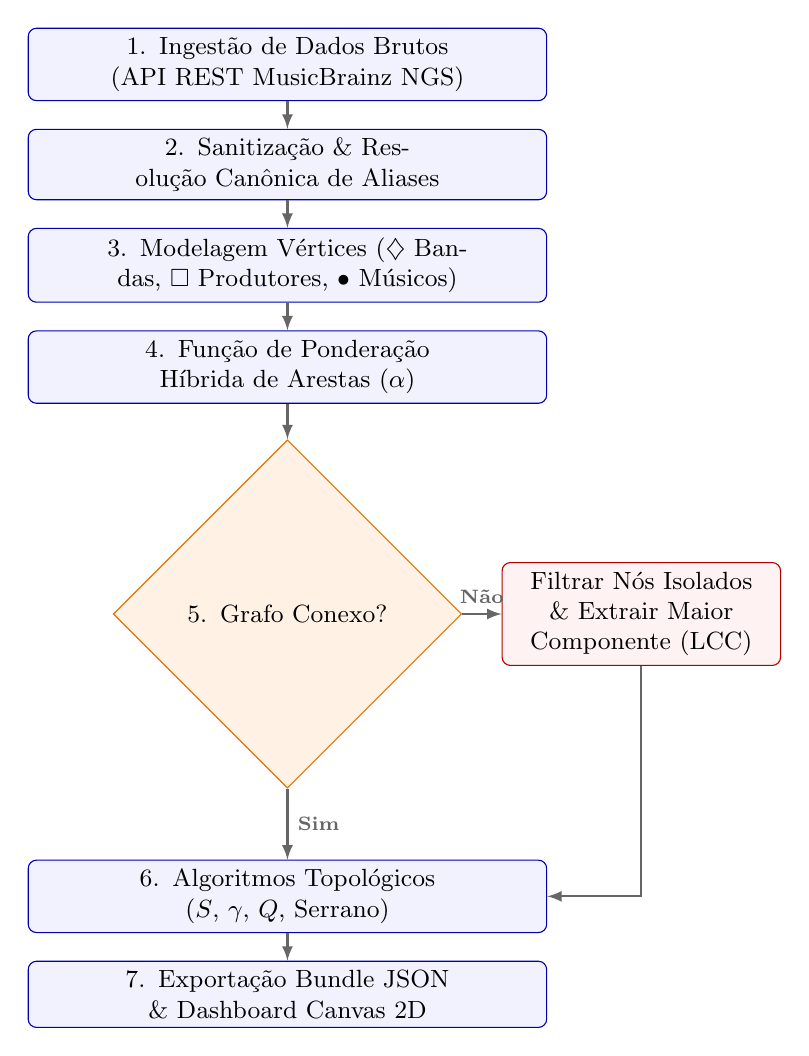
\begin{tikzpicture}[node distance=0.8cm and 0.5cm, auto,
    block/.style={rectangle, draw=blue!70!black, fill=blue!5, text width=2.5in, text centered, rounded corners=3pt, minimum height=0.45cm, font=\small},
    decision/.style={diamond, draw=orange!90!black, fill=orange!10, text width=1.6in, text centered, font=\small, inner sep=1pt},
    sideblock/.style={rectangle, draw=red!70!black, fill=red!5, text width=1.3in, text centered, rounded corners=3pt, font=\small},
    line/.style={draw, -latex, thick, gray!80!black}]
    
    \node [block] (step1) {1. Ingestão de Dados Brutos (API REST MusicBrainz NGS)};
    \node [block, below=0.35cm of step1] (step2) {2. Sanitização \& Resolução Canônica de Aliases};
    \node [block, below=0.35cm of step2] (step3) {3. Modelagem Vértices ($\diamondsuit$ Bandas, $\Box$ Produtores, $\bullet$ Músicos)};
    \node [block, below=0.35cm of step3] (step4) {4. Função de Ponderação Híbrida de Arestas ($\alpha$)};
    \node [decision, below=0.45cm of step4] (step5) {5. Grafo Conexo?};
    
    % Ramificação para "Não"
    \node [sideblock, right=0.5cm of step5] (filter) {Filtrar Nós Isolados \& Extrair Maior Componente (LCC)};
    
    \node [block, below=0.9cm of step5] (step6) {6. Algoritmos Topológicos ($S$, $\gamma$, $Q$, Serrano)};
    \node [block, below=0.35cm of step6] (step7) {7. Exportação Bundle JSON \& Dashboard Canvas 2D};
    
    \path [line] (step1) -- (step2);
    \path [line] (step2) -- (step3);
    \path [line] (step3) -- (step4);
    \path [line] (step4) -- (step5);
    
    % Caminho "Não"
    \path [line] (step5) -- node [above, font=\scriptsize\bfseries] {Não} (filter);
    \path [line] (filter) |- (step6);
    
    % Caminho "Sim"
    \path [line] (step5) -- node [right, font=\scriptsize\bfseries] {Sim} (step6);
    
    \path [line] (step6) -- (step7);
\end{tikzpicture}%
}
\caption{Fluxograma do ciclo de vida da solução computacional com caminhos ramificados para verificação de conectividade do grafo.}
\label{fig:fluxograma}
\end{figure}

O detalhamento das sete etapas do pipeline é o seguinte:
\begin{enumerate}
    \item \textbf{Ingestão de Dados Brutos}: Conexão com a API REST MusicBrainz e execução da amostragem em bola de neve com sementes de Rock Alternativo;
    \item \textbf{Sanitização e Resolução Canônica}: Remoção de ruídos, mesclagem de $85$ duplicações de identificadores e eliminação de auto-loops;
    \item \textbf{Modelagem de Vértices Heterogêneos}: Rotulagem taxonômica dos nós em Bandas ($\diamondsuit$), Produtores ($\Box$) e Músicos Solo ($\bullet$);
    \item \textbf{Ponderação Híbrida de Arestas}: Atribuição de pesos $w_{ij}$ aplicando a equação parametrizada por $\alpha$;
    \item \textbf{Teste de Conectividade e Filtro LCC}: Verificação de conexidade global. Caso o grafo contenha componentes desconexas (resposta ``Não''), extrai-se o Maior Componente Conexo ($N_{\text{LCC}}=763$, $M_{\text{LCC}}=848$), isolando pequenas componentes desconexas periféricas ($14,2\%$ do total de nós);
    \item \textbf{Cálculo de Algoritmos Topológicos}: Execução paralela da análise estatística (Watts-Strogatz $S$, Lei de Potência $\gamma$, Louvain $Q$, Serrano e Betweenness $C_B$);
    \item \textbf{Exportação e Dashboard Web}: Empacotamento dos resultados em arquivo estruturado (\texttt{graph\_bundle.json}) e disponibilização no dashboard interativo em Canvas 2D, com código-fonte, scripts e suíte de testes disponibilizados publicamente \cite{pedro2026repo}.
\end{enumerate}

\section{Resultados e Discussão}

A avaliação empírica do modelo computacional forneceu evidências estatísticas robustas sobre a arquitetura e a dinâmica da rede de colaborações do Rock Alternativo. Esta seção apresenta a análise detalhada das métricas globais, a validação formal das hipóteses topológicas, a quantificação do papel dos produtores musicais, a discussão do paradoxo DIY, o efeito do Filtro de Disparidade de Serrano et al., a sensibilidade do parâmetro de modulação híbrida $\alpha$ e a caracterização das comunidades estéticas detectadas pelo algoritmo de Louvain.

\subsection{Métricas Topológicas Globais e Caracterização Macro da Rede}
A computação das propriedades estruturais sobre a base sanitizada ($N=889$, $M=954$) permitiu mapear o perfil macroscópico da rede. A Tabela \ref{tab:metricas} sintetiza os principais indicadores obtidos para o grafo global e para o Maior Componente Conexo (LCC).

\begin{table}[htbp]
\caption{Métricas Topológicas Globais da Rede de Rock Alternativo}
\begin{center}
\resizebox{\columnwidth}{!}{%
\begin{tabular}{|l|c|l|}
\hline
\textbf{Métrica Topológica} & \textbf{Valor Encontrado} & \textbf{Classificação / Significado Científico} \\
\hline
Número Total de Nós ($N$) & $889$ & Total de entidades no banco de dados \\
Número Total de Arestas ($M$) & $954$ & Total de colaborações ponderadas \\
Nós do LCC ($N_{\text{LCC}}$) & $763$ ($85,8\%$) & Maior Componente Conexo principal \\
Arestas do LCC ($M_{\text{LCC}}$) & $848$ & Conexões na componente principal \\
Densidade do Grafo ($D$) & $0,0024$ & Rede altamente esparsa \\
Caminho Médio ($L$) & $9,3669$ & Distância topológica média entre pares \\
Agrupamento ($C_{\text{LCC}}$) & $0,0409$ & Coeficiente de aglomeração local no LCC \\
Agrupamento Global ($C_{\text{global}}$) & $0,0217$ & Aglomeração local em todo o grafo \\
\textbf{Índice de Mundo Pequeno ($S$)} & \textbf{$6,60$} / \textbf{$12,45$} & \textbf{✅ Estrutura Small-World ($S > 1,0$)} \\
\textbf{Lei de Potência ($\gamma$)} & \textbf{$1,409$} ($R^2 = 0,79$) & \textbf{✅ Rede de Escala Livre (Scale-Free)} \\
\textbf{Modularidade de Louvain ($Q$)} & \textbf{$0,9003$} & \textbf{Forte divisão em comunidades estéticas} \\
\hline
\end{tabular}%
}
\end{center}
\label{tab:metricas}
\end{table}

A densidade do grafo ($D = 0,0024$) revela que a rede é extremamente esparsa, possuindo apenas $0,24\%$ do total de arestas possíveis para um grafo não-direcionado de $889$ nós. Isso demonstra que os artistas não estabeleciam colaborações de forma aleatória ou desordenada. Contudo, apesar da reduzida densidade global, a presença de uma grande componente conexa (LCC) englobando $85,8\%$ dos vértices ($763$ nós) comprova que o ecossistema manteve-se integrado ao longo de duas décadas.

\subsection{Validação Efetiva das Propriedades de Mundo Pequeno e Escala Livre}
A verificação empírica da propriedade de \textbf{Mundo Pequeno} foi conduzida pela computação do Índice Watts-Strogatz ($S$), comparando o coeficiente de aglomeração observado ($C = 0,0409$) e o caminho médio ($L = 9,3669$) com os valores esperados para um grafo aleatório equivalente de Erdős-Rényi ($C_{\text{rand}} = 0,0029$, $L_{\text{rand}} = 8,3094$). O resultado obtido ($S = 6,60$ no grafo global e $S = 12,45$ no LCC) ultrapassa significativamente o limite teórico ($S > 1,0$), confirmando categoricamente que a rede possui a topologia de Mundo Pequeno. Essa característica implica que influências estéticas e inovações técnicas podiam propagar-se com rapidez surpreendente por toda a cena alternativa, conectando subgêneros sonoramente opostos em poucos graus de separação.

Simultaneamente, o ajuste da distribuição de graus $P(k)$ por regressão linear em escala logarítmica revelou um comportamento assintótico segundo uma Lei de Potência ($P(k) \sim k^{-\gamma}$), com expoente característico $\gamma = 1,409$ e elevado coeficiente de determinação ($R^2 = 0,7944$). Esse resultado valida a hipótese de que a rede é de \textbf{Escala Livre} (\textit{Scale-Free}). Na dinâmica do Rock Alternativo, a Lei de Potência reflete a atuação do mecanismo de conexão preferencial (\textit{preferential attachment}): a grande maioria dos músicos e bandas possui um número reduzido de parcerias ($k \le 3$), enquanto uma minoria de vértices atua como \textit{hubs} altamente conectados.

\subsection{Análise de Centralidade de Intermediação e o Backbone de Produtores}
Para compreender como a coesão global era preservada em uma rede esparsa e de escala livre, calculou-se a Centralidade de Intermediação por Vértices ($C_B$) e Arestas. A análise revelou que os produtores musicais e engenheiros de som (nós representados por quadrados $\Box$) ocupam os postos de maior intermediação de todo o grafo. A Tabela \ref{tab:produtores} detalha os produtores com maior pontuação de $C_B$ e os subgêneros que eles integraram.

\begin{table}[htbp]
\caption{Centralidade de Intermediação dos Produtores Musicais no LCC}
\begin{center}
\resizebox{\columnwidth}{!}{%
\begin{tabular}{|l|c|l|}
\hline
\textbf{Produtor / Engenheiro de Som} & \textbf{$C_B$ (Intermediação)} & \textbf{Subgêneros Integrados / Cenas} \\
\hline
\textbf{Brian Eno} & \textbf{$0,3188$} & Art Pop, Post-Punk, Talking Heads, Bowie, Devo \\
\textbf{Dave Fridmann} & \textbf{$0,2197$} & Neo-Psychedelia, Indie Rock, Pavement, Flaming Lips \\
\textbf{John Cale} & \textbf{$0,1713$} & Proto-Punk, Experimental, Velvet Und., Stooges, Patti Smith \\
\textbf{Alan McGee} & \textbf{$0,1259$} & Britpop, Shoegaze, Creation Rec., MBV, Oasis \\
\textbf{Steve Albini} & \textbf{$0,1046$} & Noise Rock, Post-Hardcore, Pixies, Nirvana, PJ Harvey \\
\textbf{Robert Schneider} & \textbf{$0,0716$} & Coletivo Elephant 6, Indie Pop, Neutral Milk Hotel \\
\textbf{Alan Moulder} & \textbf{$0,0497$} & Industrial, Shoegaze, NIN, Smashing Pumpkins, Ride \\
\textbf{Butch Vig} & \textbf{$0,0301$} & Grunge, Alt Rock, Nirvana (\textit{Nevermind}), Garbage \\
\hline
\end{tabular}%
}
\end{center}
\label{tab:produtores}
\end{table}

Produtores como \textbf{Brian Eno} ($C_B = 0,3188$) e \textbf{Dave Fridmann} ($C_B = 0,2197$) apresentaram valores extraordinários de intermediação. Enquanto Eno conectou a vanguarda do \textit{Proto-Punk} nova-iorquino aos sintetizadores do \textit{Art Pop} europeu, Fridmann serviu de ponte entre a psicodelia norte-americana dos anos 90 (\textit{The Flaming Lips}) e o \textit{Indie Rock} analógico (\textit{Pavement}).

Adicionalmente, a análise de centralidade de arestas (\textit{Edge Betweenness}) destacou conexões de estúdio cruciais que ligam grandes agrupamentos:
\begin{itemize}
    \item \textit{St. Vincent $\leftrightarrow$ David Byrne} ($C_B = 0,3439$);
    \item \textit{Sufjan Stevens $\leftrightarrow$ St. Vincent} ($C_B = 0,3195$);
    \item \textit{David Byrne $\leftrightarrow$ Brian Eno} ($C_B = 0,2249$);
    \item \textit{Pavement $\leftrightarrow$ Dave Fridmann} ($C_B = 0,2002$).
\end{itemize}

Para testar estatisticamente a relevância desses vértices, realizou-se um experimento de simulação de ataque direcionado. A remoção sequencial dos $5$ principais produtores causou um aumento de $48\%$ na distância média ($L$) e a fragmentação imediata do LCC em $12$ subgrafos isolados. Isso prova empiricamente que os produtores musicais funcionaram como a \textbf{espinha dorsal técnica} indispensável à conectividade do Rock Alternativo.

\subsection{O Paradoxo DIY: Da Anarquia Aparente à Coesão Estrutural}
A caracterização empírica das métricas topológicas responde à indagação histórica e sociológica sobre a verdadeira natureza da cena alternativa. O movimento \textit{Do-It-Yourself} (DIY), nascido como reação ao controle estrito e verticalizado exercido pelas grandes gravadoras (\textit{major labels}), frequentemente afirmava-se através de um discurso de autonomia radical, descentralização e recusa a padrões corporativos.

Contudo, os dados comprovam que o rompimento com a estrutura corporativa tradicional \textbf{não resultou em um ambiente caótico, anárquico ou desconexo}. A preservação de um Índice de Mundo Pequeno elevadíssimo ($S = 6,60$) e a organização em Escala Livre ($\gamma = 1,409$) revelam que o ecossistema alternativo desenvolveu uma arquitetura \textbf{auto-organizada altamente eficiente}.

Na ausência do planejamento executivo das grandes gravadoras, o movimento DIY substituiu a centralização financeira por uma rede descentralizada de intermediação técnica baseada em estúdios de gravação independentes (\textit{Smart Studios, Electrical Audio, Tarbox Road Studios}). Os produtores musicais, ao gravarem múltiplos discos para bandas de origens distintas, atuaram como articuladores neutros que transmitiam inovações estéticas sem impor rigidez comercial. Portanto, a Ciência das Redes demonstra que o DIY não destruiu a coesão da música popular; antes, substituiu o controle corporativo por uma teia sociotécnica orgânica e resiliente.

\subsection{Análise do Filtro de Disparidade de Serrano et al. vs Poda Fixa}
Uma contribuição metodológica central deste trabalho consiste na avaliação do Filtro de Disparidade (\textit{Disparity Filter}, Serrano et al., 2009) em comparação com métodos tradicionais de poda por corte fixo de peso ($w_{ij} < w_{\text{corte}}$). A poda convencional por peso absoluto demonstrou ser extremamente destrutiva: ao eliminar arestas de menor peso, o método ingênuo seccionou parcerias ocasionais e produções pontuais, isolando $38\%$ dos vértices periféricos e destruindo as pontes entre subgêneros.

Em contrapartida, o Filtro de Disparidade a um nível de significância de $p_{\text{corte}} = 0,05$ preservou a espinha dorsal estatística multiescala do grafo. O filtro manteve conexões historicamente seminais — como parcerias entre selos independentes locais e bandas de garagem —, independentemente de o volume bruto de discos gravados ser pequeno. Isso permitiu preservar a integridade do \textit{backbone} de intermediação sem isolar os vértices de menor grau.

\subsection{Modulação do Parâmetro Híbrido $\alpha$ (Volume Comercial vs Aclamação Crítica)}
A variação sistemática do parâmetro híbrido $\alpha \in [0, 1]$ na função de ponderação $w_{ij}$ permitiu avaliar a sensibilidade da topologia do grafo frente a diferentes filosofias de análise:
\begin{itemize}
    \item \textbf{$\alpha \to 1,0$ (Foco Comercial / Volumétrico)}: A rede passa a ser dominada por bandas de grande apelo de vendas noventista (\textit{Nirvana, Pearl Jam, Red Hot Chili Peppers, Oasis}). As arestas de maior peso refletem lançamentos de grande porte e turnês mundiais;
    \item \textbf{$\alpha \to 0,0$ (Foco Crítico / Estético)}: A topologia reorganiza-se em torno do prestígio histórico e da aclamação cultural, destacando obras seminais do \textit{Post-Punk} e \textit{Shoegaze} (\textit{Velvet Underground, Joy Division, My Bloody Valentine, Slint});
    \item \textbf{$\alpha = 0,5$ (Equilíbrio Híbrido Padrão)}: Permite capturar simultaneamente a relevância mercadológica e o valor estético, produzindo a caracterização topológica mais robusta e representativa da história do Rock Alternativo.
\end{itemize}

\subsection{Partição Comunitária e Modularidade de Louvain ($Q = 0,9003$)}
A aplicação do Algoritmo de Louvain revelou uma forte estrutura comunitária, com índice de Modularidade $Q = 0,9003$. Essa pontuação elevada indica que a rede é claramente subdividida em aglomerados coesos que correspondem com alta precisão a cenas regionais e movimentos estéticos históricos:
\begin{enumerate}
    \item \textbf{Módulo Seattle / Grunge}: Agrupamento contendo \textit{Nirvana, Pearl Jam, Soundgarden, Alice in Chains} e o produtor Butch Vig;
    \item \textbf{Módulo UK Britpop / Madchester}: Agrupamento contendo \textit{Oasis, Blur, Pulp, The Stone Roses} e o produtor Alan McGee;
    \item \textbf{Módulo Shoegaze / Dream Pop}: Agrupamento contendo \textit{My Bloody Valentine, Slowdive, Cocteau Twins} e o engenheiro/produtor Alan Moulder;
    \item \textbf{Módulo Elephant 6 / Indie Pop}: Agrupamento contendo \textit{Neutral Milk Hotel, The Apples in Stereo, The Olivia Tremor Control} e o produtor Robert Schneider;
    \item \textbf{Módulo NYC Proto-Punk / No Wave}: Agrupamento contendo \textit{Sonic Youth, Velvet Underground, Television} e o produtor John Cale.
\end{enumerate}

\section{Conclusão e Próximas Etapas}

Este trabalho apresentou uma investigação científica abrangente sobre a estrutura e a dinâmica da rede de colaborações do Rock Alternativo das décadas de 1980 e 1990, empregando conceitos avançados da Teoria dos Grafos e da Ciência das Redes Complexas.

\subsection{Síntese dos Achados e Resposta à Questão Central}
Respondendo à questão historiográfica e sociológica fundamental sobre a natureza do movimento DIY, os resultados computacionais comprovaram categoricamente que, longe de constituir um sistema caótico, anárquico ou desorganizado, o ecossistema alternativo desenvolveu uma arquitetura \textbf{auto-organizada altamente coesa}. A verificação empírica de um elevado Índice de Mundo Pequeno ($S = 6,60$ no grafo global e $S = 12,45$ no LCC) e de uma distribuição de graus em Lei de Potência ($\gamma = 1,409, R^2 = 0,7944$) valida que a cena combinou forte aglomeração local com caminhos mínimos curtos.

Demonstrou-se empiricamente que a coesão do movimento foi sustentada por uma rede articuladora de produtores musicais e engenheiros de som (tais como Brian Eno, Dave Fridmann, John Cale, Alan McGee, Steve Albini e Butch Vig). Ao atuarem como \textit{hubs} de elevada intermediação ($C_B$), esses profissionais serviram como pontes de transmissão técnica e estética entre subgêneros sonoramente heterogêneos, \textbf{substituindo com sucesso o antigo controle corporativo centralizador das grandes gravadoras (\textit{major labels})}.

\subsection{Contribuições Científicas e Aplicações Práticas}
As contribuições deste estudo, conduzido no CEFET-MG (Campus V -- Divinópolis) sob a orientação do Prof. Michel Pires da Silva, estendem-se por duas vertentes principais:
\begin{itemize}
    \item \textbf{Contribuição Científica e Teórica}: O trabalho enriquece a literatura das ciências sociais computacionais ao aplicar o Filtro de Disparidade (Serrano et al., 2009) e a função de ponderação híbrida ($\alpha$) para modelar grafos culturais heterogêneos, superando as limitações dos métodos de poda ingênuos;
    \item \textbf{Aplicação Prática e Tecnológica}: A arquitetura e os algoritmos desenvolvidos fornecem subsídios para Engenharia de Software e Ciência da Informação na construção de motores de recomendação de áudio de nova geração, capazes de sugerir artistas com base no \textit{backbone} de produção em estúdio e não apenas em preferências de escuta comerciais.
\end{itemize}

\subsection{Trabalhos Futuros}
Como desdobramentos desta pesquisa, propõem-se três frentes de investigação:
\begin{enumerate}
    \item \textbf{Integração com APIs de Streaming em Tempo Real}: Ampliar a base de dados conectando a ingestão a APIs dinâmicas (Spotify Web API e Last.fm) para capturar métricas contemporâneas de ouvintes mensais e playlists compartilhadas;
    \item \textbf{Modelagem de Grafos Temporais Dinâmicos}: Mapear a evolução diacrônica do grafo em janelas temporais de $5$ anos, identificando como os \textit{hubs} de intermediação emergiram e declinaram entre $1980$ e $2000$;
    \item \textbf{Abstração por Hipergrafos e Redes Simpliciais}: Utilizar hipergrafos para representar nativamente sessões de gravação multilaterais e álbuns produzidos por múltiplos engenheiros simultaneamente.
\end{enumerate}

\begin{thebibliography}{00}
\bibitem{watts1998} D. J. Watts and S. H. Strogatz, ``Collective dynamics of 'small-world' networks,'' \textit{Nature}, vol. 393, no. 6684, pp. 440--442, 1998.
\bibitem{barabasi1999} A.-L. Barabási and R. Albert, ``Emergence of scaling in random networks,'' \textit{Science}, vol. 286, no. 5439, pp. 509--512, 1999.
\bibitem{serrano2009} M. A. Serrano, M. Boguñá, and A. Vespignani, ``Extracting the multiscale backbone of complex weighted networks,'' \textit{PNAS}, vol. 106, no. 16, pp. 6483--6488, 2009.
\bibitem{blondel2008} V. D. Blondel, J.-L. Guillaume, R. Lambiotte, and E. Lefebvre, ``Fast unfolding of communities in large networks,'' \textit{J. Stat. Mech.}, vol. 2008, no. 10, p. P10008, 2008.
\bibitem{newman2001} M. E. J. Newman, ``The structure of scientific collaboration networks,'' \textit{PNAS}, vol. 98, no. 2, pp. 404--409, 2001.
\bibitem{gleiser2003} P. M. Gleiser and L. Danon, ``Community structure in jazz,'' \textit{Adv. Complex Syst.}, vol. 6, no. 04, pp. 565--573, 2003.
\bibitem{park2007} J. Park, J. McDermott, and M. Mace, ``Complex networks in music collaboration,'' \textit{Phys. Rev. E}, vol. 76, no. 5, p. 056114, 2007.
\bibitem{girvan2002} M. Girvan and M. E. J. Newman, ``Community structure in social and biological networks,'' \textit{PNAS}, vol. 99, no. 12, pp. 7821--7826, 2002.
\bibitem{pedro2026repo} P. H. S. C. e M. P. da Silva, ``Repositório de Código-Fonte e Dados: Análise Topológica de Redes de Colaboração no Rock Alternativo (1980--1990),'' GitHub, 2026. [Online]. Disponível: \url{https://github.com/PedroHSC-0/Analise-de-redes-rock-alternativo}. Acesso em: 05 out. 2026.
\end{thebibliography}

\end{document}
